\documentclass{beamer}
\usetheme{Berlin}

% \setbeamertemplate{background canvas}[vertical shading][bottom=white,top=structure.fg!25]

\usepackage[utf8]{inputenc}
\usepackage[ngerman]{babel} %% neue rechtschreibung
%\usepackage[german]
\usepackage[T1]{fontenc}
\usepackage{times}
%\usepackage{bigdelim}
\usecolortheme{whale}
\usepackage{xcolor}
\usepackage{listings} %Quellcode einbinden

\beamertemplatenavigationsymbolsempty

\useoutertheme{infolines}

\title{SciServer}
\subtitle{ Entwicklung einer Serversoftware zur Verwaltung von
	wissenschaftlichen Daten}
\author{Jens Kapitza}
\date{November 2015}
\subject{Informatik}

% Falls Aufzhlungen immer schrittweise gezeigt werden sollen, kann
% folgendes Kommando benutzt werden:
% \beamerdefaultoverlayspecification{<+->}
\usepackage{multicol}

\begin{document}
	
	
\section{Einführung}
\begin{frame}
	\titlepage
\end{frame}

\begin{frame}[shrink,allowdisplaybreaks]{Gliederung}
  \tableofcontents[subsectionstyle=hide]
\end{frame}


\begin{frame}{Thema}
\begin{block}{Wissenschaftliche Daten}
\begin{itemize}
	\item Sehr große Dateien
	\item Unbekannte Dateitypen
	\item Öffentlich, Lizenzen/Patente
	\item Sehr viele Dateien
\end{itemize}
\end{block}


\begin{block}{Aktionen}
	\begin{itemize}
		\item Anlegen
		\item Verwalten (Attribute, Schlagwörter)
		\item Verteilen
		\item Suchen
	\end{itemize}
\end{block}

\end{frame}

\section{Problemstellung und Lösungsansätze}

\begin{frame}[shrink]{Gliederung}
	\tableofcontents[currentsection,hideothersubsections]{}	
\end{frame}

\subsection{Einführung}
\begin{frame}{Probleme}
 
 \begin{block}{Betriebssysteme}
 	\begin{itemize}
 		\item nicht einheitlich (Programme und Benutzerinterfacekonzepte)
 		\item unterstützen nicht alles (Schlagwortbegrenzung, Dateigrößen)
 		\item Protokolle weichen untereinander ab (Limitierungen HTTP)
 	\end{itemize}
 \end{block}
 
 \begin{block}{Ziele}
 		\begin{itemize}
 		\item Verwaltung und Suchen über Tags und Attribute
 		\item Vorverarbeitung wie Prüfsummen, Filtervorgänge
 		\item Benachrichtigungen
 		\item Verteilen von Dateien
 	\end{itemize}
 \end{block}
 
\end{frame}


\begin{frame}

\begin{block}{Anforderungen}
	\begin{itemize}
		\item Plattform unabhängig 
		\item Weboberfläche zum Suchen und Verwalten
		\item Einfach, einfach, einfach.
	\end{itemize}
\end{block}

\begin{block}{Java-Stack}
	\begin{itemize}
		\item JSF, JMS, JPA, CDI
		\item JVM, Vorteil oder Nachteil?
	\end{itemize}
\end{block}



\end{frame}



\subsection{Cloud-Ansatz}


\begin{frame}[shrink]{Cloud-Ansatz}
	
	\begin{block}{Möglichkeiten}
		\begin{itemize}
			\item Dropbox 
			\item Windows One Drive
			\item Google Drive, \ldots
		\end{itemize}
		
	\end{block}
	 
	
	
	\begin{block}{Optionen}
		\begin{itemize}
			\item Verteilung der Daten
			\item Zentrale Speicherung
			\item Weboberfläche und ggf. Client
		\end{itemize}
		
		
	\end{block}
	
	
	\begin{block}{Bedenken}
		\begin{multicols}{2}
			\begin{itemize}
				\item Rechtlich? 
				\item Datenspeicherung?
				\item Unterstützung?
				\item Kosten?
				\item Informationen teilen?
				\item Informationen verwalten?
				\item Informationen suchen?
				\item Informationszugriff?
			\end{itemize}		
		\end{multicols}
	\end{block}
	
	\bigskip
	
\end{frame}




\subsection{,,private Cloud''-Ansatz}



\begin{frame}[shrink]{,,private Cloud''-Ansatz}
	
	\begin{block}{Möglichkeiten}
		\begin{itemize}
			\item Owncloud 
			\item Horde
			\item FTP, HTTP, NFS, \ldots
		\end{itemize}
		
	\end{block}
	
	\begin{block}{Optionen}
		\begin{itemize}
			\item Verteilung der Daten (manuell)
			\item Zentrale Speicherung
			\item Weboberfläche meist keine Clients
		\end{itemize}
		
		
	\end{block}
	
	
	\begin{block}{Bedenken}
		\begin{multicols}{2}
			\begin{itemize}
				\item Rechtlich? 
				\item Datenspeicherung?
				\item Unterstützung?
				\item Kosten?
				\item Informationen teilen?
				\item Informationen verwalten?
				\item Informationen suchen?
				\item Informationszugriff?
			\end{itemize}		
		\end{multicols}
	\end{block}
	
	\bigskip
	
\end{frame}

\subsection{Dokumenten Management System (DMS)}


\begin{frame}[shrink]{Dokumenten Management System (DMS)}
	
	\begin{block}{Möglichkeiten}
		\begin{itemize}
			\item openKM 
			\item Alfresco One
		\end{itemize}
		
	\end{block}
	
	\begin{block}{Optionen}
		\begin{itemize}
			\item Verteilung der Daten
			\item Zentrale Speicherung
			\item Weboberfläche und spezielle Clients als Addon
		\end{itemize}
		
		
	\end{block}
	
	
	\begin{block}{Bedenken}
		\begin{multicols}{2}
		\begin{itemize}
			\item Rechtlich? 
			\item Datenspeicherung?
			\item Unterstützung?
			\item Kosten?
			\item Informationen teilen?
			\item Informationen verwalten?
			\item Informationen suchen?
			\item Informationszugriff?
			\end{itemize}		
		\end{multicols}
	\end{block}
	
	\bigskip
	
\end{frame}



\subsection{Peer-to-Peer Ansatz}



\begin{frame}[shrink]{Peer-to-Peer Ansatz}
	
	\begin{block}{Möglichkeiten}
		\begin{itemize}
			\item Napster, \ldots
			\item SciServer
		\end{itemize}
		
	\end{block}
	
	\begin{block}{Optionen}
		\begin{itemize}
			\item Verteilung der Daten
			\item \textbf{Dezentrale Speicherung}
			\item Weboberfläche und Agenten
		\end{itemize}
		
		
	\end{block}
	
	
	\begin{block}{Bedenken}
		\begin{multicols}{2}
			\begin{itemize}
				\item Rechtlich? 
				\item Datenspeicherung?
				\item Unterstützung?
				\item Kosten?
				\item Informationen teilen?
				\item Informationen verwalten?
				\item Informationen suchen?
				\item Informationszugriff?
			\end{itemize}		
		\end{multicols}
	\end{block}
	
	
	\bigskip
	
\end{frame}



\section{Strukturen und Kommunikationsmuster im Lösungsansatz}

\begin{frame}[shrink]{Gliederung}
	\tableofcontents[currentsection,hideothersubsections]{}	
\end{frame}



\subsection{Strukturen für Peers / Smart-Hosts / Proxys }


\begin{frame}{Strukturen}
	
	
	\begin{description}
		\item[Client-Server] Weboberfläche nutzt HTML und HTTP. Diese bindet Browser an.\\
		Mailclient wird durch die ,,database'' und den Benachrichtigungen durch IMAP und SMTP angebunden.\\
				
		\item[Peer-to-Peer]  einfach: Jeder redet mit jedem und ist jedem anderem gleich gestellt.\\
		 Aber: einzelne Peers erledigen als Agenten bestimmte Aufgaben.\\
		 Das System kann einfach wachsen, indem weitere Anwendungen gestartet werden.
		 \item[Publish-Subscribe] Kommunikation wird an alle angemeldeten Peers verteilt. 
		 vgl. Bus-System, Observer-Pattern, Vermittler
	\end{description}
	 
\end{frame}


\subsection{Agenten im Peer-to-Peer}


\begin{frame}{Agenten im Peer-to-Peer}
 
	 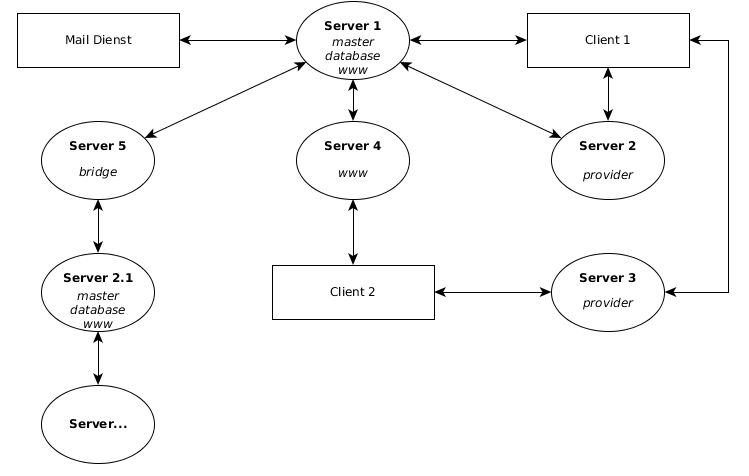
\includegraphics[width=\textwidth]{clients_uebersicht.png}
	 
	
\end{frame}




\subsection{Systembefehle und Arbeiten mit Dateien}


 

\begin{frame}{Arbeiten mit Dateien}
	
	
	\begin{block}{Java-Stack}
	\begin{description}
		\item[Files, Path] Zugriff auf die Informationen einer Datei 
		\item[WatchService] Überwachen der Änderungen in einem Ordner\\Aber: nicht wer die Änderung gemacht hat (Prozess), sondern nur, dass Änderungen passiert sind.
		\item[Prozesse] Plattform unabhängig, Aber kaum Informationen über Prozesse 'generalisiert' möglich.
		\item[Netzwerk, JMS] Nutzung von Javas interner Serialisierung. Bibliotheken haben Memory-Leaks und Abstürze.
	 
	\end{description}
\end{block}
 
\end{frame}


\section{Version 2.0}


\begin{frame}
	
	
	\begin{block}{TODOs}
		\begin{description}
			\item[Prozesse] Möglichkeit bieten, auf Informationen der gestarteten Prozesse sowie deren Fortschritt zu verfolgen.
			\item[Netzwerk] Kommunikation anpassen auf SSH. \\
			Einen eigenen Server bereitstellen (mit Benutzer/Peer Verwaltung) unabhängig vom Betriebssystem.
			\item[Web] Migration auf einen kleineren Webserver.\\
			Ein Applicationserver bietet mehr als die Anwendung brauch, jedoch ein einfacher Webcontainer zu wenig.
			
		
			\end{description}
	\end{block}
	
	\bigskip 
	
	
\end{frame}

\begin{frame}
	
	
	\begin{block}{TODOs}
		\begin{description}
				
			\item[WatchService] Versuch herauszufinden welcher Prozess die Änderungen gemacht hat.\\
			Bessere Benachrichtigungen.
			
			
			
			\item[Mail-Client] 
			Einen eigenen Agenten für Benachrichtigungen und Interaktion mit dem System schreiben.
			\item[Client-Anwendung]
			Viele Funktionen können nicht ohne Desktop-Anwendung ausgeführt werden, die Sicherheitsbeschränkungen in HTML
			können je nach Browser nur schwer umgangen werden. Das ist nicht praktikabel! Daher ist eine Desktop-Anwendung besser für einige Funktionen geeignet.
			
			
		\end{description}
	\end{block}
	
	\bigskip 
	
	
\end{frame}


\section{DEMO (interaktiv)}

\begin{frame}
	
	
	\begin{exampleblock}{DEMO}	\begin{itemize}
			\item Starten des Master, Database, Provider und WWW
			\item Suchen einer Datei
			\item Taggen einer Datei
			\item Benachrichtigungen (für E-Mail, Internet nötig)
			\item Ausführung eines Filters/Befehls
			
		\end{itemize}
	\end{exampleblock}

	
\end{frame}

\begin{frame}{Fragen?}
	\begin{block}{}
		\begin{quote}
			
			
Wer nicht danke sagen kann,\\
wird irgendwann vergeblich bitten. \\
– Fred Ammon, http://www.aphorismen.de
		\end{quote}

	\end{block}
	
	\bigskip
	 
\end{frame}

\end{document}


